% Options for packages loaded elsewhere
\PassOptionsToPackage{unicode}{hyperref}
\PassOptionsToPackage{hyphens}{url}
\PassOptionsToPackage{dvipsnames,svgnames,x11names}{xcolor}
%
\documentclass[
  ignorenonframetext,
]{beamer}
\usepackage{pgfpages}
\setbeamertemplate{caption}[numbered]
\setbeamertemplate{caption label separator}{: }
\setbeamercolor{caption name}{fg=normal text.fg}
\beamertemplatenavigationsymbolsempty
% Prevent slide breaks in the middle of a paragraph
\widowpenalties 1 10000
\raggedbottom
\setbeamertemplate{part page}{
  \centering
  \begin{beamercolorbox}[sep=16pt,center]{part title}
    \usebeamerfont{part title}\insertpart\par
  \end{beamercolorbox}
}
\setbeamertemplate{section page}{
  \centering
  \begin{beamercolorbox}[sep=12pt,center]{part title}
    \usebeamerfont{section title}\insertsection\par
  \end{beamercolorbox}
}
\setbeamertemplate{subsection page}{
  \centering
  \begin{beamercolorbox}[sep=8pt,center]{part title}
    \usebeamerfont{subsection title}\insertsubsection\par
  \end{beamercolorbox}
}
\AtBeginPart{
  \frame{\partpage}
}
\AtBeginSection{
  \ifbibliography
  \else
    \frame{\sectionpage}
  \fi
}
\AtBeginSubsection{
  \frame{\subsectionpage}
}
\usepackage{amsmath,amssymb}
\usepackage{lmodern}
\usepackage{iftex}
\ifPDFTeX
  \usepackage[T1]{fontenc}
  \usepackage[utf8]{inputenc}
  \usepackage{textcomp} % provide euro and other symbols
\else % if luatex or xetex
  \usepackage{unicode-math}
  \defaultfontfeatures{Scale=MatchLowercase}
  \defaultfontfeatures[\rmfamily]{Ligatures=TeX,Scale=1}
\fi
% Use upquote if available, for straight quotes in verbatim environments
\IfFileExists{upquote.sty}{\usepackage{upquote}}{}
\IfFileExists{microtype.sty}{% use microtype if available
  \usepackage[]{microtype}
  \UseMicrotypeSet[protrusion]{basicmath} % disable protrusion for tt fonts
}{}
\makeatletter
\@ifundefined{KOMAClassName}{% if non-KOMA class
  \IfFileExists{parskip.sty}{%
    \usepackage{parskip}
  }{% else
    \setlength{\parindent}{0pt}
    \setlength{\parskip}{6pt plus 2pt minus 1pt}}
}{% if KOMA class
  \KOMAoptions{parskip=half}}
\makeatother
\usepackage{xcolor}
\newif\ifbibliography
\usepackage{color}
\usepackage{fancyvrb}
\newcommand{\VerbBar}{|}
\newcommand{\VERB}{\Verb[commandchars=\\\{\}]}
\DefineVerbatimEnvironment{Highlighting}{Verbatim}{commandchars=\\\{\}}
% Add ',fontsize=\small' for more characters per line
\usepackage{framed}
\definecolor{shadecolor}{RGB}{248,248,248}
\newenvironment{Shaded}{\begin{snugshade}}{\end{snugshade}}
\newcommand{\AlertTok}[1]{\textcolor[rgb]{0.94,0.16,0.16}{#1}}
\newcommand{\AnnotationTok}[1]{\textcolor[rgb]{0.56,0.35,0.01}{\textbf{\textit{#1}}}}
\newcommand{\AttributeTok}[1]{\textcolor[rgb]{0.77,0.63,0.00}{#1}}
\newcommand{\BaseNTok}[1]{\textcolor[rgb]{0.00,0.00,0.81}{#1}}
\newcommand{\BuiltInTok}[1]{#1}
\newcommand{\CharTok}[1]{\textcolor[rgb]{0.31,0.60,0.02}{#1}}
\newcommand{\CommentTok}[1]{\textcolor[rgb]{0.56,0.35,0.01}{\textit{#1}}}
\newcommand{\CommentVarTok}[1]{\textcolor[rgb]{0.56,0.35,0.01}{\textbf{\textit{#1}}}}
\newcommand{\ConstantTok}[1]{\textcolor[rgb]{0.00,0.00,0.00}{#1}}
\newcommand{\ControlFlowTok}[1]{\textcolor[rgb]{0.13,0.29,0.53}{\textbf{#1}}}
\newcommand{\DataTypeTok}[1]{\textcolor[rgb]{0.13,0.29,0.53}{#1}}
\newcommand{\DecValTok}[1]{\textcolor[rgb]{0.00,0.00,0.81}{#1}}
\newcommand{\DocumentationTok}[1]{\textcolor[rgb]{0.56,0.35,0.01}{\textbf{\textit{#1}}}}
\newcommand{\ErrorTok}[1]{\textcolor[rgb]{0.64,0.00,0.00}{\textbf{#1}}}
\newcommand{\ExtensionTok}[1]{#1}
\newcommand{\FloatTok}[1]{\textcolor[rgb]{0.00,0.00,0.81}{#1}}
\newcommand{\FunctionTok}[1]{\textcolor[rgb]{0.00,0.00,0.00}{#1}}
\newcommand{\ImportTok}[1]{#1}
\newcommand{\InformationTok}[1]{\textcolor[rgb]{0.56,0.35,0.01}{\textbf{\textit{#1}}}}
\newcommand{\KeywordTok}[1]{\textcolor[rgb]{0.13,0.29,0.53}{\textbf{#1}}}
\newcommand{\NormalTok}[1]{#1}
\newcommand{\OperatorTok}[1]{\textcolor[rgb]{0.81,0.36,0.00}{\textbf{#1}}}
\newcommand{\OtherTok}[1]{\textcolor[rgb]{0.56,0.35,0.01}{#1}}
\newcommand{\PreprocessorTok}[1]{\textcolor[rgb]{0.56,0.35,0.01}{\textit{#1}}}
\newcommand{\RegionMarkerTok}[1]{#1}
\newcommand{\SpecialCharTok}[1]{\textcolor[rgb]{0.00,0.00,0.00}{#1}}
\newcommand{\SpecialStringTok}[1]{\textcolor[rgb]{0.31,0.60,0.02}{#1}}
\newcommand{\StringTok}[1]{\textcolor[rgb]{0.31,0.60,0.02}{#1}}
\newcommand{\VariableTok}[1]{\textcolor[rgb]{0.00,0.00,0.00}{#1}}
\newcommand{\VerbatimStringTok}[1]{\textcolor[rgb]{0.31,0.60,0.02}{#1}}
\newcommand{\WarningTok}[1]{\textcolor[rgb]{0.56,0.35,0.01}{\textbf{\textit{#1}}}}
\usepackage{graphicx}
\makeatletter
\def\maxwidth{\ifdim\Gin@nat@width>\linewidth\linewidth\else\Gin@nat@width\fi}
\def\maxheight{\ifdim\Gin@nat@height>\textheight\textheight\else\Gin@nat@height\fi}
\makeatother
% Scale images if necessary, so that they will not overflow the page
% margins by default, and it is still possible to overwrite the defaults
% using explicit options in \includegraphics[width, height, ...]{}
\setkeys{Gin}{width=\maxwidth,height=\maxheight,keepaspectratio}
% Set default figure placement to htbp
\makeatletter
\def\fps@figure{htbp}
\makeatother
\setlength{\emergencystretch}{3em} % prevent overfull lines
\providecommand{\tightlist}{%
  \setlength{\itemsep}{0pt}\setlength{\parskip}{0pt}}
\setcounter{secnumdepth}{-\maxdimen} % remove section numbering
\usepackage{graphicx}
\usepackage{bm}
\usepackage{array}
\usepackage{amsmath}
\usepackage{amsthm}
\usepackage{amsfonts}
\usepackage{amssymb}
\usepackage{tikz-cd}
\usepackage{url}
\definecolor{foreground}{RGB}{255,255,255}
\definecolor{background}{RGB}{34,28,54}
\definecolor{title}{RGB}{105,165,255}
\definecolor{gray}{RGB}{175,175,175}
\definecolor{lightgray}{RGB}{225,225,225}
\definecolor{subtitle}{RGB}{232,234,255}
\definecolor{hilight}{RGB}{112,224,255}
\definecolor{vhilight}{RGB}{255,111,207}
\setbeamertemplate{footline}[page number]
\ifLuaTeX
  \usepackage{selnolig}  % disable illegal ligatures
\fi
\IfFileExists{bookmark.sty}{\usepackage{bookmark}}{\usepackage{hyperref}}
\IfFileExists{xurl.sty}{\usepackage{xurl}}{} % add URL line breaks if available
\urlstyle{same} % disable monospaced font for URLs
\hypersetup{
  pdftitle={STAT 528 - Advanced Regression Analysis II},
  pdfauthor={Multinomial response regression (part I)},
  colorlinks=true,
  linkcolor={Maroon},
  filecolor={Maroon},
  citecolor={Blue},
  urlcolor={blue},
  pdfcreator={LaTeX via pandoc}}

\title{STAT 528 - Advanced Regression Analysis II}
\author{Multinomial response regression (part I)}
\date{}
\institute{Daniel J. Eck\\
Department of Statistics\\
University of Illinois}

\begin{document}
\frame{\titlepage}

\begin{frame}
\newcommand{\R}{\mathbb{R}}
\newcommand{\Prob}{\mathbb{P}}
\newcommand{\Proj}{\textbf{P}}
\newcommand{\Hcal}{\mathcal{H}}
\newcommand{\rootn}{\sqrt{n}}
\newcommand{\p}{\mathbf{p}}
\newcommand{\E}{\text{E}}
\newcommand{\Var}{\text{Var}}
\newcommand{\Cov}{\text{Cov}}
\newcommand{\mubf}{\bm{\mu}}
\newcommand{\logit}{\text{logit}}

\newtheorem{cor}{Corollary}
\newtheorem{lem}{Lemma}
\newtheorem{thm}{Theorem}
\newtheorem{defn}{Definition}
\newtheorem{prop}{Proposition}
\end{frame}

\begin{frame}{Last time}
\protect\hypertarget{last-time}{}
\begin{itemize}
\tightlist
\item
  Overdispersion
\item
  Gala data analysis
\item
  Negative Binomial regression
\item
  Zero Inflated Count Models
\end{itemize}
\end{frame}

\begin{frame}{Learning Objectives Today}
\protect\hypertarget{learning-objectives-today}{}
\begin{itemize}
\tightlist
\item
  Multinomial regression via baseline-category logistic model
\item
  Data analysis
\end{itemize}

\vspace{12pt}

This slide deck will be a little bit different. It will only contain the
data analysis. The lecture will be largely on the blackboard.
\end{frame}

\begin{frame}{Baseball example}
\protect\hypertarget{baseball-example}{}
In the game of baseball it is important to understand how the
characteristics of a player's swing translate to positive outcomes on
the baseball field. We want to estimate the probabilities of different
baseball outcomes given quality of swing and hitting tendency variables
(obtained by STATCAST).

\vspace{12pt}

The outcomes of interest are:

\begin{itemize}
\tightlist
\item
  single (1 base)
\item
  double (2 bases)
\item
  triple (3 bases)
\item
  home runs (4 bases)
\item
  and outs (0 bases; taken as baseline)
\end{itemize}
\end{frame}

\begin{frame}{}
\protect\hypertarget{section}{}
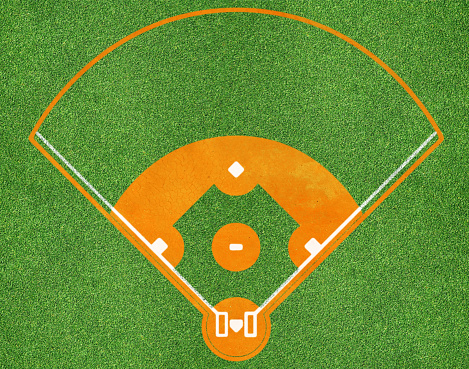
\includegraphics{baseballfield.jpg}
\end{frame}

\begin{frame}{}
\protect\hypertarget{section-1}{}
The more bases the better, 4 bases = 1 run.

\vspace{12pt}

The team with the most runs wins the game. An out (0 bases) is a bad
outcome for a batter, an out means the batter ended their time at the
plate without reaching base.

\vspace{12pt}

We want to estimate the probabilities of singles, doubles, triples, home
runs, and outs as a function of swing and batting tendency variables
are:

\begin{itemize}
\tightlist
\item
  exit velocity (launch speed off the bat)
\item
  launch angle (angle off the bat into the air)
\item
  spray angle (where on the field the ball is going)
\end{itemize}
\end{frame}

\begin{frame}{}
\protect\hypertarget{section-2}{}
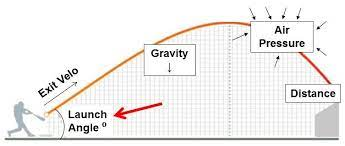
\includegraphics{la.jpg}
\end{frame}

\begin{frame}{}
\protect\hypertarget{section-3}{}
We will use the baseline-category logistic model for this example. We
encoded events so that outs is the baseline category.

\vspace{12pt}

We will build models using AIC, LRT, and domain knowledge.
\end{frame}

\begin{frame}[fragile]{}
\protect\hypertarget{section-4}{}
We now load in the relevant software and data set and display the first
10 rows of the data set

\vspace{12pt}
\tiny

\begin{Shaded}
\begin{Highlighting}[]
\FunctionTok{library}\NormalTok{(VGAM)  }\CommentTok{\# has model{-}fitting functions}
\NormalTok{bball }\OtherTok{\textless{}{-}} \FunctionTok{read.csv}\NormalTok{(}\StringTok{"bball.csv"}\NormalTok{)}
\NormalTok{bball}\SpecialCharTok{$}\NormalTok{events }\OtherTok{\textless{}{-}} \FunctionTok{as.factor}\NormalTok{(bball}\SpecialCharTok{$}\NormalTok{events)}
\FunctionTok{dim}\NormalTok{(bball)}
\end{Highlighting}
\end{Shaded}

\begin{verbatim}
## [1] 50000     6
\end{verbatim}

\begin{Shaded}
\begin{Highlighting}[]
\FunctionTok{head}\NormalTok{(bball, }\DecValTok{10}\NormalTok{)}
\end{Highlighting}
\end{Shaded}

\begin{verbatim}
##    pitcher batter events launch_speed launch_angle spray_angle
## 1   623167 493329    out         82.3          -41   2.4599306
## 2   592761 573131     b2         95.9           22 -12.0705545
## 3   429722 592206     b2        101.0           13 -45.5422457
## 4   571760 621005    out         61.9           63  12.9786747
## 5   519008 663757    out         93.2            5 -40.1840254
## 6   456501 672695    out         95.3           26  -9.4373687
## 7   605182 521692    out         74.9           35  -3.1754445
## 8   502624 444482    out         57.9          -28  -0.5256346
## 9   596133 595777    out         96.8          -23  45.8961936
## 10  579328 545358     b4        101.9           28  -0.9735690
\end{verbatim}
\end{frame}

\begin{frame}{}
\protect\hypertarget{section-5}{}
We will fit two baseline category logistic models (nested) using a
\texttt{vglm} from the \texttt{VGAM} package.

\vspace{12pt}

One of these models contains a square term for launch angle, why?
\end{frame}

\begin{frame}{}
\protect\hypertarget{section-6}{}
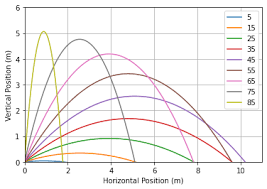
\includegraphics{la_var.png}
\end{frame}

\begin{frame}{}
\protect\hypertarget{section-7}{}
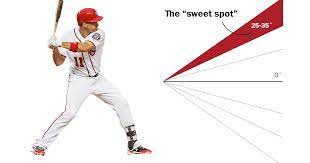
\includegraphics{la_sweet.jpg}
\end{frame}

\begin{frame}[fragile]{}
\protect\hypertarget{section-8}{}
The model with a quadratic term for launch angle fits the data better.

\vspace{12pt}
\tiny

\begin{Shaded}
\begin{Highlighting}[]
\NormalTok{mod1 }\OtherTok{\textless{}{-}} \FunctionTok{vglm}\NormalTok{(events }\SpecialCharTok{\textasciitilde{}}\NormalTok{ launch\_speed }\SpecialCharTok{+}\NormalTok{ launch\_angle }\SpecialCharTok{+}\NormalTok{ spray\_angle, }
             \AttributeTok{family=}\NormalTok{multinomial, }\AttributeTok{data=}\NormalTok{bball)}
\FunctionTok{system.time}\NormalTok{(mod2 }\OtherTok{\textless{}{-}} \FunctionTok{vglm}\NormalTok{(events }\SpecialCharTok{\textasciitilde{}}\NormalTok{ launch\_speed }\SpecialCharTok{+}\NormalTok{ launch\_angle }\SpecialCharTok{+}\NormalTok{ spray\_angle }\SpecialCharTok{+} 
               \FunctionTok{I}\NormalTok{(launch\_angle}\SpecialCharTok{\^{}}\DecValTok{2}\NormalTok{), }
             \AttributeTok{family=}\NormalTok{multinomial, }\AttributeTok{data=}\NormalTok{bball))}
\end{Highlighting}
\end{Shaded}

\begin{verbatim}
##    user  system elapsed 
##   2.622   0.303   2.925
\end{verbatim}

\begin{Shaded}
\begin{Highlighting}[]
\FunctionTok{AIC}\NormalTok{(mod2) }
\end{Highlighting}
\end{Shaded}

\begin{verbatim}
## [1] 70914.6
\end{verbatim}

\begin{Shaded}
\begin{Highlighting}[]
\FunctionTok{AIC}\NormalTok{(mod1)}
\end{Highlighting}
\end{Shaded}

\begin{verbatim}
## [1] 83119.98
\end{verbatim}

\begin{Shaded}
\begin{Highlighting}[]
\FunctionTok{pchisq}\NormalTok{(}\FunctionTok{deviance}\NormalTok{(mod2), }\FunctionTok{df.residual}\NormalTok{(mod2), }\AttributeTok{lower =} \ConstantTok{FALSE}\NormalTok{)}
\end{Highlighting}
\end{Shaded}

\begin{verbatim}
## [1] 1
\end{verbatim}
\end{frame}

\begin{frame}[fragile]{}
\protect\hypertarget{section-9}{}
Model fitting is slow. Let's try scaling the predictors. Scaling does
not change the model but it may speed up the optimization.

\vspace{12pt}
\tiny

\begin{Shaded}
\begin{Highlighting}[]
\NormalTok{bball\_scale }\OtherTok{\textless{}{-}}\NormalTok{ bball}
\NormalTok{bball\_scale[, }\DecValTok{4}\SpecialCharTok{:}\DecValTok{6}\NormalTok{] }\OtherTok{\textless{}{-}} \FunctionTok{scale}\NormalTok{(bball[, }\DecValTok{4}\SpecialCharTok{:}\DecValTok{6}\NormalTok{])}

\FunctionTok{system.time}\NormalTok{(mod2\_scale }\OtherTok{\textless{}{-}} \FunctionTok{vglm}\NormalTok{(events }\SpecialCharTok{\textasciitilde{}}\NormalTok{ launch\_speed }\SpecialCharTok{+}\NormalTok{ launch\_angle }\SpecialCharTok{+} 
\NormalTok{    spray\_angle }\SpecialCharTok{+}  \FunctionTok{I}\NormalTok{(launch\_angle}\SpecialCharTok{\^{}}\DecValTok{2}\NormalTok{), }
    \AttributeTok{family=}\NormalTok{multinomial, }\AttributeTok{data=}\NormalTok{bball\_scale))}
\end{Highlighting}
\end{Shaded}

\begin{verbatim}
##    user  system elapsed 
##   2.534   0.296   2.832
\end{verbatim}

\begin{Shaded}
\begin{Highlighting}[]
\FunctionTok{round}\NormalTok{(}\FunctionTok{AIC}\NormalTok{(mod2), }\DecValTok{4}\NormalTok{) }\SpecialCharTok{==} \FunctionTok{round}\NormalTok{(}\FunctionTok{AIC}\NormalTok{(mod2\_scale), }\DecValTok{4}\NormalTok{)}
\end{Highlighting}
\end{Shaded}

\begin{verbatim}
## [1] TRUE
\end{verbatim}
\end{frame}

\begin{frame}{}
\protect\hypertarget{section-10}{}
What type of polynomial should we consider for spray angle?
\end{frame}

\begin{frame}{}
\protect\hypertarget{section-11}{}
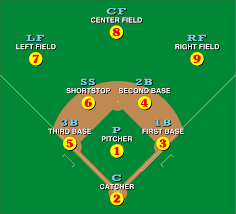
\includegraphics{positions.png}
\end{frame}

\begin{frame}[fragile]{}
\protect\hypertarget{section-12}{}
How about a 6th order polynomial?

\vspace{12pt}
\tiny

\begin{Shaded}
\begin{Highlighting}[]
\FunctionTok{system.time}\NormalTok{(mod3 }\OtherTok{\textless{}{-}} \FunctionTok{vglm}\NormalTok{(events }\SpecialCharTok{\textasciitilde{}}\NormalTok{ launch\_speed }\SpecialCharTok{+}\NormalTok{ launch\_angle }\SpecialCharTok{+}\NormalTok{ spray\_angle }\SpecialCharTok{+} 
               \FunctionTok{I}\NormalTok{(launch\_angle}\SpecialCharTok{\^{}}\DecValTok{2}\NormalTok{) }\SpecialCharTok{+} \FunctionTok{I}\NormalTok{(spray\_angle}\SpecialCharTok{\^{}}\DecValTok{2}\NormalTok{) }\SpecialCharTok{+} \FunctionTok{I}\NormalTok{(spray\_angle}\SpecialCharTok{\^{}}\DecValTok{3}\NormalTok{) }\SpecialCharTok{+} 
               \FunctionTok{I}\NormalTok{(spray\_angle}\SpecialCharTok{\^{}}\DecValTok{4}\NormalTok{) }\SpecialCharTok{+} \FunctionTok{I}\NormalTok{(spray\_angle}\SpecialCharTok{\^{}}\DecValTok{5}\NormalTok{) }\SpecialCharTok{+} \FunctionTok{I}\NormalTok{(spray\_angle}\SpecialCharTok{\^{}}\DecValTok{6}\NormalTok{),}
             \AttributeTok{family=}\NormalTok{multinomial, }\AttributeTok{data=}\NormalTok{bball))}
\end{Highlighting}
\end{Shaded}

\begin{verbatim}
##    user  system elapsed 
##   8.624   0.689   9.317
\end{verbatim}

\begin{Shaded}
\begin{Highlighting}[]
\FunctionTok{system.time}\NormalTok{(mod3\_scale }\OtherTok{\textless{}{-}} \FunctionTok{vglm}\NormalTok{(events }\SpecialCharTok{\textasciitilde{}}\NormalTok{ launch\_speed }\SpecialCharTok{+}\NormalTok{ launch\_angle }\SpecialCharTok{+}\NormalTok{ spray\_angle }\SpecialCharTok{+} 
               \FunctionTok{I}\NormalTok{(launch\_angle}\SpecialCharTok{\^{}}\DecValTok{2}\NormalTok{) }\SpecialCharTok{+} \FunctionTok{I}\NormalTok{(spray\_angle}\SpecialCharTok{\^{}}\DecValTok{2}\NormalTok{) }\SpecialCharTok{+} \FunctionTok{I}\NormalTok{(spray\_angle}\SpecialCharTok{\^{}}\DecValTok{3}\NormalTok{) }\SpecialCharTok{+} 
               \FunctionTok{I}\NormalTok{(spray\_angle}\SpecialCharTok{\^{}}\DecValTok{4}\NormalTok{) }\SpecialCharTok{+} \FunctionTok{I}\NormalTok{(spray\_angle}\SpecialCharTok{\^{}}\DecValTok{5}\NormalTok{) }\SpecialCharTok{+} \FunctionTok{I}\NormalTok{(spray\_angle}\SpecialCharTok{\^{}}\DecValTok{6}\NormalTok{), }
             \AttributeTok{family=}\NormalTok{multinomial, }\AttributeTok{data=}\NormalTok{bball\_scale))}
\end{Highlighting}
\end{Shaded}

\begin{verbatim}
##    user  system elapsed 
##   8.091   0.549   8.640
\end{verbatim}

\vspace{12pt}
\normalsize

Scaling the predictors did not dramatically improve computational time.
\end{frame}

\begin{frame}[fragile]{}
\protect\hypertarget{section-13}{}
Our 6th order polynomial model for spray angle fits the data better than
the model with a single linear term.

\vspace{12pt}
\tiny

\begin{Shaded}
\begin{Highlighting}[]
\FunctionTok{AIC}\NormalTok{(mod3); }\FunctionTok{AIC}\NormalTok{(mod2)}
\end{Highlighting}
\end{Shaded}

\begin{verbatim}
## [1] 66678.96
\end{verbatim}

\begin{verbatim}
## [1] 70914.6
\end{verbatim}

\begin{Shaded}
\begin{Highlighting}[]
\FunctionTok{pchisq}\NormalTok{(}\FunctionTok{deviance}\NormalTok{(mod3), }\FunctionTok{df.residual}\NormalTok{(mod3), }\AttributeTok{lower =} \ConstantTok{FALSE}\NormalTok{)}
\end{Highlighting}
\end{Shaded}

\begin{verbatim}
## [1] 1
\end{verbatim}

\vspace{12pt}
\normalsize

We could try larger polynomial models, but numerical precision becomes
problematic. Scaling did not alleviate this issue.
\end{frame}

\begin{frame}[fragile]{}
\protect\hypertarget{section-14}{}
We now consider some interaction terms.

\vspace{12pt}
\tiny

\begin{Shaded}
\begin{Highlighting}[]
\FunctionTok{system.time}\NormalTok{(mod4 }\OtherTok{\textless{}{-}} \FunctionTok{vglm}\NormalTok{(events }\SpecialCharTok{\textasciitilde{}}\NormalTok{ launch\_speed }\SpecialCharTok{+}\NormalTok{ launch\_angle }\SpecialCharTok{+}\NormalTok{ spray\_angle }\SpecialCharTok{+} 
               \FunctionTok{I}\NormalTok{(launch\_angle}\SpecialCharTok{\^{}}\DecValTok{2}\NormalTok{) }\SpecialCharTok{+} 
               \FunctionTok{I}\NormalTok{(spray\_angle}\SpecialCharTok{\^{}}\DecValTok{2}\NormalTok{) }\SpecialCharTok{+} \FunctionTok{I}\NormalTok{(spray\_angle}\SpecialCharTok{\^{}}\DecValTok{3}\NormalTok{) }\SpecialCharTok{+} \FunctionTok{I}\NormalTok{(spray\_angle}\SpecialCharTok{\^{}}\DecValTok{4}\NormalTok{) }\SpecialCharTok{+} 
               \FunctionTok{I}\NormalTok{(spray\_angle}\SpecialCharTok{\^{}}\DecValTok{5}\NormalTok{) }\SpecialCharTok{+} \FunctionTok{I}\NormalTok{(spray\_angle}\SpecialCharTok{\^{}}\DecValTok{6}\NormalTok{) }\SpecialCharTok{+} 
               \FunctionTok{I}\NormalTok{(spray\_angle}\SpecialCharTok{*}\NormalTok{launch\_angle) }\SpecialCharTok{+} \FunctionTok{I}\NormalTok{(spray\_angle}\SpecialCharTok{*}\NormalTok{launch\_speed) }\SpecialCharTok{+} 
               \FunctionTok{I}\NormalTok{(launch\_angle}\SpecialCharTok{*}\NormalTok{launch\_speed), }
             \AttributeTok{family=}\NormalTok{multinomial, }\AttributeTok{data=}\NormalTok{bball))}
\end{Highlighting}
\end{Shaded}

\begin{verbatim}
##    user  system elapsed 
##   9.150   0.598   9.761
\end{verbatim}

\begin{Shaded}
\begin{Highlighting}[]
\FunctionTok{AIC}\NormalTok{(mod3); }\FunctionTok{AIC}\NormalTok{(mod4)}
\end{Highlighting}
\end{Shaded}

\begin{verbatim}
## [1] 66678.96
\end{verbatim}

\begin{verbatim}
## [1] 66325.19
\end{verbatim}

\begin{Shaded}
\begin{Highlighting}[]
\FunctionTok{pchisq}\NormalTok{(}\FunctionTok{deviance}\NormalTok{(mod4), }\FunctionTok{df.residual}\NormalTok{(mod4), }\AttributeTok{lower =} \ConstantTok{FALSE}\NormalTok{)}
\end{Highlighting}
\end{Shaded}

\begin{verbatim}
## [1] 1
\end{verbatim}
\end{frame}

\begin{frame}[fragile]{}
\protect\hypertarget{section-15}{}
Let's now examine what we can do with this flexible final model.

\vspace{12pt}

We plot the \(\log\left(\frac{\hat\pi_j(x)}{\hat\pi_J(x)}\right)\) as a
function of spray angle for each hit outcome where \(J\) corresponds to
an out.

\vspace{12pt}

We will set launch angle and exit velocity to their median values.

\vspace{12pt}
\tiny

\begin{Shaded}
\begin{Highlighting}[]
\FunctionTok{summary}\NormalTok{(bball}\SpecialCharTok{$}\NormalTok{launch\_angle)}
\end{Highlighting}
\end{Shaded}

\begin{verbatim}
##    Min. 1st Qu.  Median    Mean 3rd Qu.    Max. 
##  -89.00   -6.00   12.00   12.29   30.00   89.00
\end{verbatim}

\begin{Shaded}
\begin{Highlighting}[]
\FunctionTok{summary}\NormalTok{(bball}\SpecialCharTok{$}\NormalTok{launch\_speed)}
\end{Highlighting}
\end{Shaded}

\begin{verbatim}
##    Min. 1st Qu.  Median    Mean 3rd Qu.    Max. 
##    9.40   80.00   90.30   88.07   98.80  121.30
\end{verbatim}

\begin{Shaded}
\begin{Highlighting}[]
\DocumentationTok{\#\# obtain predictions}
\NormalTok{new\_data }\OtherTok{=} \FunctionTok{data.frame}\NormalTok{(}\AttributeTok{spray\_angle =} \FunctionTok{seq}\NormalTok{(}\SpecialCharTok{{-}}\DecValTok{55}\NormalTok{,}\DecValTok{55}\NormalTok{, }\AttributeTok{by =} \FloatTok{0.1}\NormalTok{), }
           \AttributeTok{launch\_speed =} \FloatTok{90.30}\NormalTok{, }
           \AttributeTok{launch\_angle =} \DecValTok{12}\NormalTok{)}
\NormalTok{pred }\OtherTok{\textless{}{-}} \FunctionTok{predict}\NormalTok{(mod4, }\AttributeTok{newdata =}\NormalTok{ new\_data)}
\FunctionTok{head}\NormalTok{(pred, }\DecValTok{3}\NormalTok{)}
\end{Highlighting}
\end{Shaded}

\begin{verbatim}
##   log(mu[,1]/mu[,5]) log(mu[,2]/mu[,5]) log(mu[,3]/mu[,5]) log(mu[,4]/mu[,5])
## 1         -0.3442213           3.755072          -1.852540          -12.67547
## 2         -0.3460507           3.737278          -1.854847          -12.68112
## 3         -0.3478719           3.719141          -1.857601          -12.68688
\end{verbatim}

\begin{Shaded}
\begin{Highlighting}[]
\NormalTok{pred2 }\OtherTok{\textless{}{-}} \FunctionTok{predict}\NormalTok{(mod4, }\AttributeTok{newdata =}\NormalTok{ new\_data, }\AttributeTok{tyoe =} \StringTok{"response"}\NormalTok{)}
\end{Highlighting}
\end{Shaded}
\end{frame}

\begin{frame}{}
\protect\hypertarget{section-16}{}
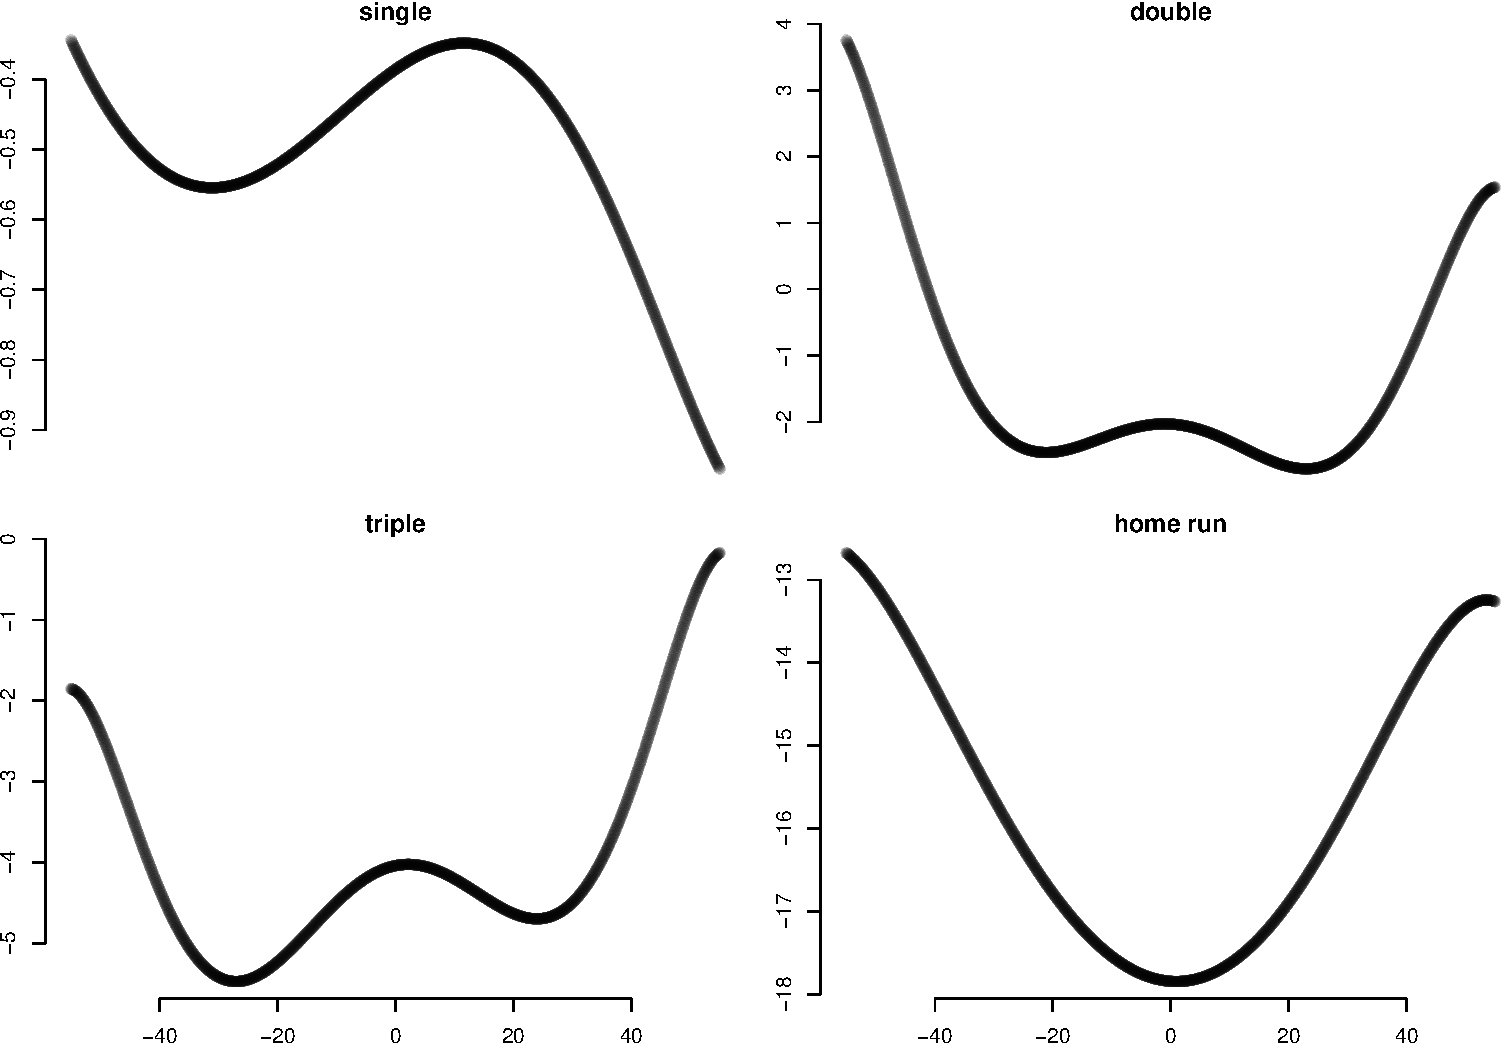
\includegraphics{week6_p1_files/figure-beamer/unnamed-chunk-4-1.pdf}
\end{frame}

\begin{frame}[fragile]{}
\protect\hypertarget{section-17}{}
Let's consider these predicted values at a new combination of launch
angle and exit velocity.

\vspace{12pt}
\tiny

\begin{Shaded}
\begin{Highlighting}[]
\DocumentationTok{\#\# obtain predictions}
\NormalTok{new\_data }\OtherTok{=} \FunctionTok{data.frame}\NormalTok{(}\AttributeTok{spray\_angle =} \FunctionTok{seq}\NormalTok{(}\SpecialCharTok{{-}}\DecValTok{55}\NormalTok{,}\DecValTok{55}\NormalTok{, }\AttributeTok{by =} \FloatTok{0.1}\NormalTok{), }
           \AttributeTok{launch\_speed =} \DecValTok{100}\NormalTok{, }
           \AttributeTok{launch\_angle =} \DecValTok{20}\NormalTok{)}
\NormalTok{pred }\OtherTok{\textless{}{-}} \FunctionTok{predict}\NormalTok{(mod4, }\AttributeTok{newdata =}\NormalTok{ new\_data)}
\FunctionTok{head}\NormalTok{(pred, }\DecValTok{3}\NormalTok{)}
\end{Highlighting}
\end{Shaded}

\begin{verbatim}
##   log(mu[,1]/mu[,5]) log(mu[,2]/mu[,5]) log(mu[,3]/mu[,5]) log(mu[,4]/mu[,5])
## 1         -0.8249607           4.777891         -0.2259619          0.7844824
## 2         -0.8263690           4.760494         -0.2284624          0.7784865
## 3         -0.8277692           4.742754         -0.2314093          0.7723810
\end{verbatim}
\end{frame}

\begin{frame}{}
\protect\hypertarget{section-18}{}
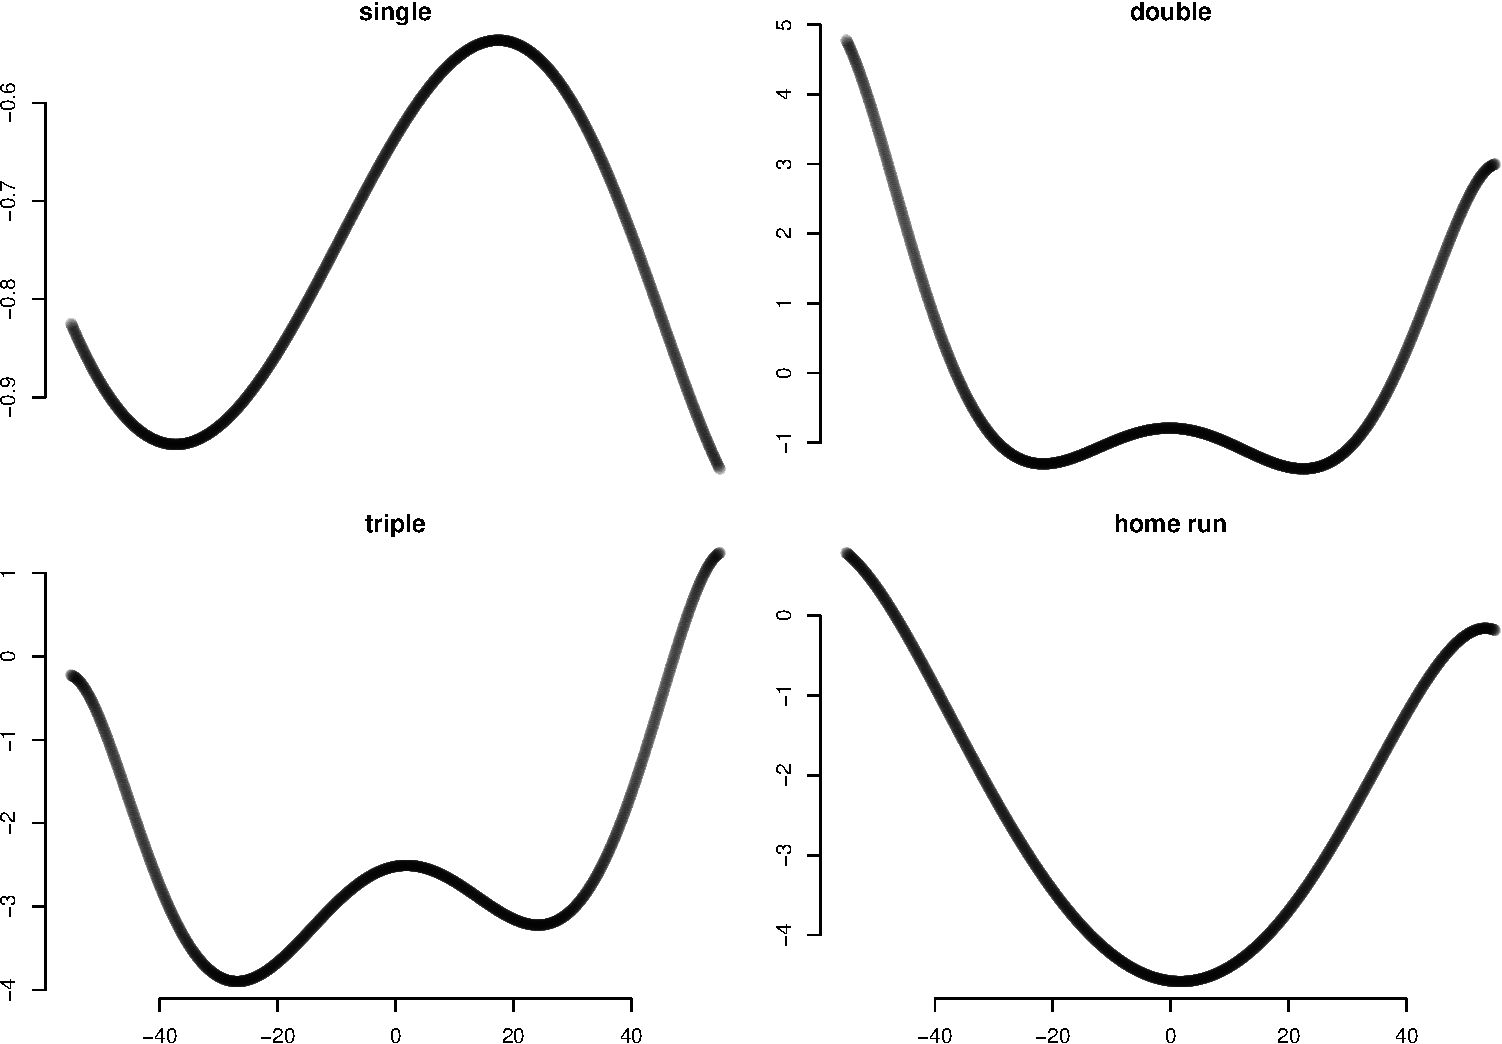
\includegraphics{week6_p1_files/figure-beamer/unnamed-chunk-6-1.pdf}
\end{frame}

\begin{frame}{Going deeper: SEAM methodology}
\protect\hypertarget{going-deeper-seam-methodology}{}
We have developed a tool for estimating batted-ball distributions for
individual batter-pitcher matchups. SEAM is shorthand for Synthetic
Estimated Average Matchup. Here is the app:

\vspace{12pt}

\url{https://seam.stat.illinois.edu/}

\vspace{12pt}

Authors:

\begin{itemize}
\tightlist
\item
  Julia Wapner (currently at Baltimore Orioles)
\item
  Charles Young (currently at Houston Astros)
\item
  David Dalpiaz
\item
  Daniel J Eck
\end{itemize}
\end{frame}

\begin{frame}{What is SEAM?}
\protect\hypertarget{what-is-seam}{}
SEAM posits a nonparametric regression model between 2-dimensional
batted-ball coordinates and the same STATCAST variables that we
considered in this lecture.

\vspace{12pt}

Matchup data is sparse. So we borrow data from ``similar'' matchups to
help estimate the batted-ball distribution under study.

\vspace{12pt}

Some methodology choices are subjective. However, SEAM performs well.

\vspace{12pt}

For more details, see here:
\url{https://github.com/ecklab/seam-manuscript/blob/main/seam.pdf}
\end{frame}

\begin{frame}{Why SEAM?}
\protect\hypertarget{why-seam}{}
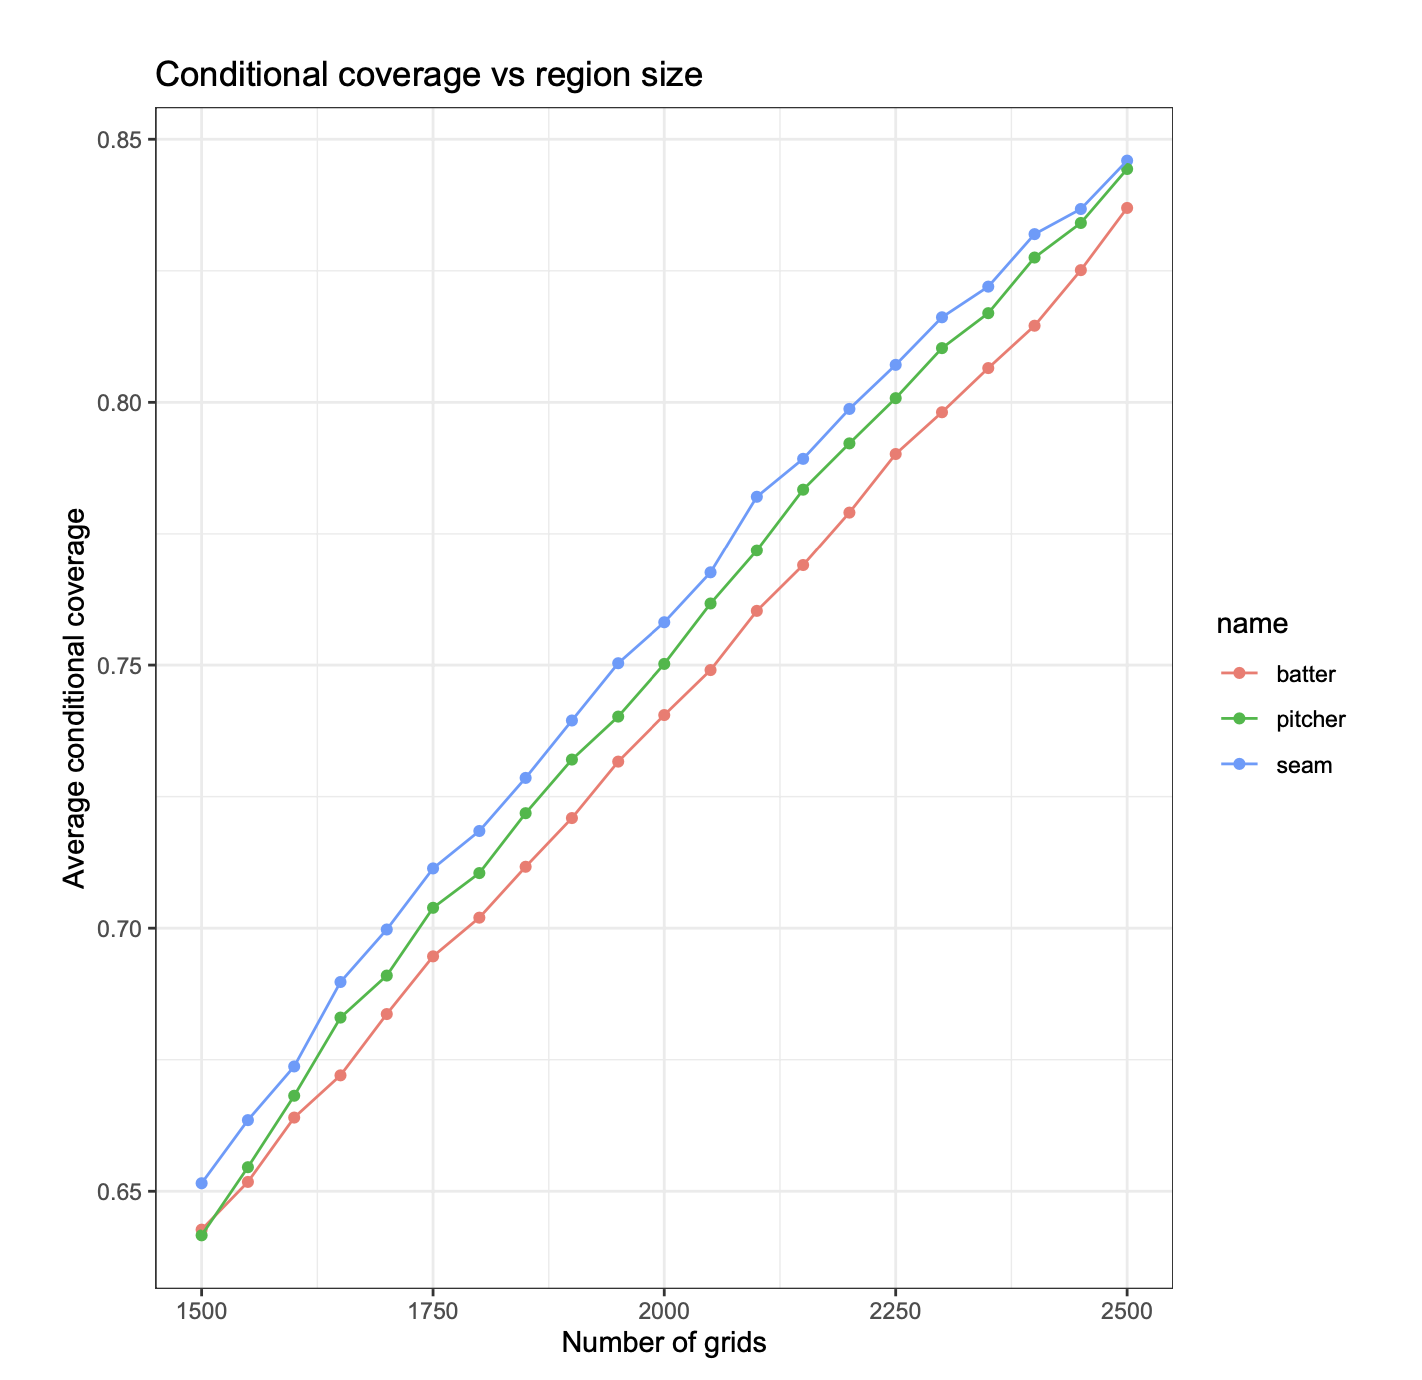
\includegraphics{seam_coverage.png}
\end{frame}

\end{document}
